\newpage
\def\thoigian{90}%--Thời gian
\de{Đề số 3}{Chương VI. Hàm số mũ và hàm số lôgarit}


\begin{center}
	\textbf{PHẦN 1 - CÂU TRẮC NGHIỆM BỐN PHƯƠNG ÁN}
\end{center}
\Opensolutionfile{ans}[ans/ans-TN-ONTAPCHUONG-DE1]
%%%==============Cau_EX1==============%%%
\begin{ex}%[1D6N1-2]%[Dự án D - đợt 4. NH24-25-Dương Công Tạo]
	Với $a$ là số thực dương tùy ý,biểu thức $\sqrt{a^3}$ được biểu diễn dưới dạng luỹ thừa của số mũ hữu tỉ là
	\choice
	{$a^6$}
	{\True $a^{\tfrac{3}{2}}$}
	{$a^{\tfrac{2}{3}}$}
	{$a^{\tfrac{1}{6}}$}
	\loigiai{
		Với $a > 0$ ta có $\sqrt{a^3}=a^{\tfrac{3}{2}}$.
	}
\end{ex}
%%%==============HetCau_EX1==============%%%

%%%==============Cau_EX2==============%%%
\begin{ex}%[1D6N1-2]%[Dự án D - đợt 4. NH24-25-Dương Công Tạo]
	Cho $a > 0$, $m$, $n\in \mathbb{R}$. Khẳng định nào sau đây đúng?
	\choice
	{$a^m+a^n=a^{m+n}$}
	{$a^m\cdot a^n=a^{m-n}$}
	{\True $(a^m)^n=(a^n)^m$}
	{$\dfrac{a^m}{a^n}=a^{n-m}$}
	\loigiai{
		Theo tính chất lũy thừa, ta có $(a^m)^n=(a^n)^m=a^{m\cdot n}$.
	}
\end{ex}
%%%==============HetCau_EX2==============%%%

%%%==============Cau_EX3==============%%%
\begin{ex}%[1D6H1-2]%[Dự án D - đợt 4. NH24-25-Dương Công Tạo]
	Rút gọn biểu thức $Q=b^{\tfrac{5}{3}}:\sqrt[3]b$ với $b > 0$.
	\choice
	{$Q=b^{-\tfrac{4}{3}}$}
	{\True $Q=b^{\tfrac{4}{3}}$}
	{$Q=b^{\tfrac{5}{9}}$}
	{$Q=b^2$}
	\loigiai{
		\[Q=b^{\tfrac{5}{3}}:\sqrt[3]b=b^{\tfrac{5}{3}}:b^{\tfrac{1}{3}}=b^{\tfrac{4}{3}}.\]
	}
\end{ex}
%%%==============HetCau_EX3==============%%%

%%%==============Cau_EX4==============%%%
\begin{ex}%[1D6H2-2]%[Dự án D - đợt 4. NH24-25-Dương Công Tạo]
	Giá trị $a^{2-3\log_a b}$ ($0< a\ne 1$, $b > 0$) bằng
	\choice
	{\True $a^2b^{-3}$}
	{$a^2b$}
	{$a^2b^3$}
	{$ab^2$}
	\loigiai{
	Ta có $a^{2-3\log_a b}=\dfrac{a^2}{a^{3\log_a b}}=\dfrac{a^2}{b^3}=a^2b^{-3}$.
	}
\end{ex}
%%%==============HetCau_EX4==============%%%

%%%==============Cau_EX5==============%%%
\begin{ex}%[1D6H2-3]%[Dự án D - đợt 4. NH24-25-Dương Công Tạo]
	Cho $a$ là số thực dương tùy ý, $\ln (9a)-\ln (7a)$ bằng?
	\choice
	{$\dfrac{\ln (9a)}{\ln (7a)}$}
	{\True $\ln \dfrac{9}{7}$}
	{$\ln (2a)$}
	{$\dfrac{\ln 9}{\ln 7}$}
	\loigiai{
		Với $a>0$, ta có $\ln (9a)-\ln (7a)=\ln \left(\dfrac{9a}{7a} \right)=\ln \dfrac{9}{7}$.
	}
\end{ex}
%%%==============HetCau_EX5==============%%%

%%%==============Cau_EX6==============%%%
\begin{ex}%[1D6H2-2]%[Dự án D - đợt 4. NH24-25-Dương Công Tạo]
	Cho $3^a=5$, khi đó $\log_{25} 81$ bằng
	\choice
	{$\dfrac{1}{2a}$}
	{$\dfrac{a}{2}$}
	{\True $\dfrac{2}{a}$}
	{$2a$}
	\loigiai{
		Ta có $3^a=5\Leftrightarrow a=\log_3 5$.\\
		Khi đó $\log _{25} 81=2\log_5 3=\dfrac{2}{\log_3 5}=\dfrac{2}{a}$.
	}
\end{ex}
%%%==============HetCau_EX6==============%%%

%%%==============Cau_EX7==============%%%
\begin{ex}%[1D6N3-2]%[Dự án D - đợt 4. NH24-25-Dương Công Tạo]
	 Tập xác định $\mathscr{D}$ của hàm số $y=\log_5 (2x+6)$ là
	\choice
	{$\mathscr{D}=\mathbb{R}$}
	{$\mathscr{D}=(3;+\infty)$}
	{\True $\mathscr{D}=(-3;+\infty)$}
	{$\mathscr{D}=\mathbb{R}\setminus \{-3\}$}
	\loigiai{
		Điều kiện xác định $2x+6> 0\Leftrightarrow x >-3$.\\
		Vậy tập xác định $\mathscr{D}=(-3;+\infty)$. 
	}
\end{ex}
%%%==============HetCau_EX7==============%%%

%%%==============Cau_EX8==============%%%
\begin{ex}%[1D6V3-3]%[Dự án D - đợt 4. NH24-25-Dương Công Tạo]
	\immini[thm]{Cho hàm số $y=a^x$ và $y=b^x$ có đồ thị như hình vẽ. Đường thẳng $y=4$ cắt trục tung, đồ thị $y=a^x$, đồ thị $y=b^x$ lần lượt tại các điểm $A$, $B$, $C$ thỏa mãn $AC=3AB$. Khẳng định nào dưới đây đúng?
		\choice
		{$a=3b$}
		{$3a=b$}
		{$a^3=b$}
		{\True $a=b^3$}}
	{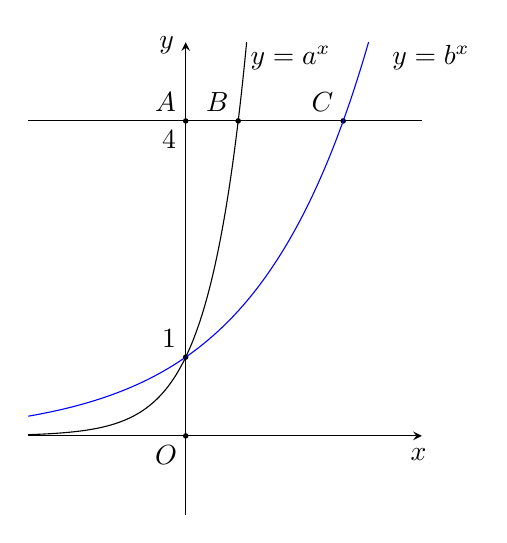
\begin{tikzpicture}[line cap=butt,line join=miter,>=stealth,font=\normalsize]
			\tikzset{declare function={xmin=-2;xmax=3;ymin=-1;ymax=5;
					f(\x)=2^(\x);
					g(\x)=8^(\x);
				},
				smooth,samples=450
			}
			\draw (xmin,4)--(xmax,4)	(0,4)node[below left]{$4$};
			\draw[->] (xmin,0)--(xmax,0) node[shift={(-100:7pt)}]{$ x $};
			\draw[->] (0,ymin)--(0,ymax) node[shift={(190:7pt)}]{$ y $};
			\fill (0,0)circle(1pt) node[shift={(225:10pt)}]{$ O $}
			(0,4)circle(1pt) node[above left]{$A$}
			(2,4)circle(1pt) node[above left]{$C$}
			(2/3,4)circle(1pt) node[above left]{$B$}
			(0,1)circle(1pt) node[above left]{$1$}
			(0.7,4.8)node[right]{$y=a^x$}
			(2.5,4.8)node[right]{$y=b^x$}
			;
			\clip (xmin,ymin) rectangle (xmax,ymax);
			\draw[blue]  plot[domain=xmin:xmax] (\x, {f(\x)});
			\draw  plot[domain=xmin:xmax] (\x, {g(\x)});
		\end{tikzpicture}
	}
	\loigiai{
		 Dựa vào hình vẽ, ta có tọa độ các điểm là $A(0;4)$, $B\left(\log_a 4;4\right)$ và $C\left(\log_b 4;4\right)$.\\
		Theo giả thiết \allowdisplaybreaks
		\begin{eqnarray*}
			AC=3AB&\Leftrightarrow& \log_b 4=3\log_a 4\\
			&\Leftrightarrow& \dfrac{1}{\log_4 b}=\dfrac{3}{\log_4 a}\\
			&\Leftrightarrow& \log_4 a=3\log_4 b\\
			&\Leftrightarrow& a=b^3.
		\end{eqnarray*}
	}
\end{ex}
%%%==============HetCau_EX8==============%%%

%%%==============Cau_EX9==============%%%
\begin{ex}%[1D6H3-5]%[Dự án D - đợt 4. NH24-25-Dương Công Tạo]
	Cường độ ánh sáng đi qua môi trường khác không khí (chẳng hạn sương mù, nước,{\dots}) sẽ giảm dần tùy thuộc độ dày của môi trường. Hằng số $\mu$ gọi là khả năng hấp thu của môi trường, tùy thuộc môi trường thì khả năng hấp thu tính theo công thức $I=I_0 \mathrm{e}^{-\mu x}$ với $x$ là độ dày của môi trường đó và được tính bằng đơn vị mét. Biết rằng nước biển có $\mu=1{,}4$. Hãy tính cường độ ánh sáng giảm đi bao nhiêu lần khi từ độ sâu $2$\,m xuống đến $20$\,m?
	\choice
	{\True $\mathrm{e}^{25{,}2}$}
	{$\mathrm{e}^{22{,}5}$}
	{$\mathrm{e}^{32{,}5}$}
	{$\mathrm{e}^{52{,}5}$}
	\loigiai{
		Cường độ ánh sáng thay đổi khi từ độ sâu $x_1$ đến độ sâu $x_2$ là
		\[\dfrac{I_1}{I_2}=\dfrac{I_0 \mathrm{e}^{-\mu x_1}}{I_0 \mathrm{e}^{-\mu x_2}}=\mathrm{e}^{\mu \left(x_2-x_1 \right)}=\mathrm{e}^{25{,}2}.\]
	}
\end{ex}
%%%==============HetCau_EX9==============%%%

%%%==============Cau_EX10==============%%%
\begin{ex}%[1D6H4-5]%[Dự án D - đợt 4. NH24-25-Dương Công Tạo]
	Tập nghiệm của bất phương trình $\log _{\tfrac{1}{2}} \left(x-3\right)\ge 2$ là
	\choice
	{$\left(-\infty;\dfrac{13}{4}\right]$}
	{$\left[\dfrac{13}{4};+\infty\right]$}
	{\True $\left(3;\dfrac{13}{4}\right]$}
	{$\left[3;\dfrac{13}{4}\right]$}
	\loigiai{
		Điều kiện xác định $x-3> 0\Leftrightarrow x > 3$.\\
		Với điều kiện trên, bất phương trình đã cho tương đương \[\log _{\tfrac{1}{2}} \left(x-3\right)\ge 2\Leftrightarrow x-3\le \left(\dfrac{1}{2} \right)^2\Leftrightarrow x\le \dfrac{13}{4}.\]
		Kết hợp với điều kiện $x > 3$, ta được $3< x\le \dfrac{13}{4}$.\\
		Vậy tập nghiệm của bất phương trình đã cho là $\left(3;\dfrac{13}{4}\right]$.
	}
\end{ex}
%%%==============HetCau_EX10==============%%%

%%%==============Cau_EX11==============%%%
\begin{ex}%[1D6N4-2]%[Dự án D - đợt 4. NH24-25-Dương Công Tạo]
	Nghiệm thực của phương trình $2^x=7$ là
	\choice
	{$x=\sqrt{7}$}
	{$x=\dfrac{7}{2}$}
	{\True $x=\log_2 7$}
	{$x=\log_7 2$}
	\loigiai{
		Ta có $2^x=7\Leftrightarrow x=\log_2 7$.
	}
\end{ex}
%%%==============HetCau_EX11==============%%%

%%%==============Cau_EX12==============%%%
\begin{ex}%[1D6H4-6]%[Dự án D - đợt 4. NH24-25-Dương Công Tạo]
	Một người gửi tiết kiệm vào ngân hàng với lãi suất $8{,}4\%$/năm và tiền lãi hàng năm được nhập vào tiền vốn. Tính số năm tối thiểu người đó cần gửi để số tiền thu được nhiều hơn $2$ lần số tiền gửi ban đầu.
	\choice
	{$10$ năm}
	{\True $9$ năm}
	{$8$ năm}
	{$11$ năm}
	\loigiai{
		Gọi số tiền gửi ban đầu là $A$ và số năm thỏa yêu cầu bài toán là $n$.\\
		Ta có $A\left(1+8{,}4\% \right)^n > 2A\Leftrightarrow 1{,}084^n > 2\Leftrightarrow n > \log _{1{,}084} 2\approx 8{,}59$.\\
		Vậy số năm tối thiểu là $9$ năm.
	}
\end{ex}
%%%==============HetCau_EX12==============%%%
\Closesolutionfile{ans}
%\begin{center}
%	\textbf{ĐÁP ÁN}
%	\inputansbox{10}{ans/ans}	
%\end{center}



\begin{center}
	\textbf{PHẦN 2 - CÂU TRẮC NGHIỆM ĐÚNG SAI}
\end{center}

\Opensolutionfile{ans}[ans/answer-DS-ONTAPCHUONG-DE1]
\setcounter{ex}{0}
%%%%==============Cau_EX1==============%%%
\begin{ex}%[1D6H2-2]%[Dự án D - đợt 4. NH24-25-Dương Công Tạo]
	Cho $a$, $b$ là các số thực dương.
	\choiceTF
		{\True $\mathrm{e}^{\ln a-\ln b}=\dfrac{a}{b}$}
		{$\ln \dfrac{a}{\sqrt[3]b}=\ln a-3\ln b$}
		{\True $\ln\left(a^2b^4\right)=2\ln (ab)+2\ln b$}
		{\True $a\ln \dfrac{1}{b}=\ln\left(b^{-a}\right)$}
	\loigiai{
		\begin{itemchoice}
			\itemch Ta có $\mathrm{e}^{\ln a-\ln b}=\mathrm{e}^{\ln \tfrac{a}{b}}=\dfrac{a}{b}$.
			\itemch $\ln \dfrac{a}{\sqrt[3]b}=\ln a-\ln \sqrt[3]b=\ln a-\ln b^{\tfrac{1}{3}}=\ln a-\dfrac{1}{3} \ln b$.
			\itemch $\ln \left(a^2b^4\right)=\ln \left(a^2b^2b^2\right)=\ln \left(ab\right)^2+\ln b^2=2\ln (ab)+2\ln b$.
			\itemch $a\ln \dfrac{1}{b}=a\ln\left(b^{-1}\right)=-a\ln b=\ln \left(b^{-a}\right)$.
		\end{itemchoice}
		}
\end{ex}
%%%%==============HetCau_EX1==============%%%

%%%==============Cau_EX2==============%%%
\begin{ex}%[1D6H3-3]%[Dự án D - đợt 4. NH24-25-Dương Công Tạo]
	Cho hàm số $y=\log_{0{,}5} x$.
	\choiceTF
	{Hàm số có tập xác định $\mathscr{D}=\mathbb{R}$}
	 {\True Hàm số nghịch biến trên khoảng $(0;+\infty)$}
	{\True Đồ thị hàm số cắt trục hoành tại điểm $A(1;0)$} 
	{\True Đồ thị hàm số đi qua điểm $N\left(\dfrac{1}{2};1\right)$}
	\loigiai{
		\begin{itemchoice}
			\itemch Hàm số $y=\log_{0{,}5} x$ xác định khi và chỉ khi $x>0$.\\
			Vậy tập xác định $\mathscr{D}=(0;+\infty)$.
			\itemch Hàm số $y=\log_{0{,}5} x$ có cơ số $a=0{,}5<1$ nên nó nghịch biến trên khoảng $(0;+\infty)$.
			\itemch Vì $\log_{0{,}5} 1=0$ nên đồ thị hàm số cắt trục hoành tại điểm $A(1;0)$.
			\itemch Vì $\log_{0{,}5} \dfrac{1}{2}=1$ nên đồ thị hàm số đi qua điểm $N\left(\dfrac{1}{2};1\right)$.
		\end{itemchoice}
}
\end{ex}
%%%==============HetCau_EX2==============%%%
\Closesolutionfile{ans}
%\inputansbox[2]{2}{ans/answer.tex}



\begin{center}
\textbf{PHẦN 3 - CÂU TRẮC NGHIỆM TRẢ LỜI NGẮN}
\end{center}
\setcounter{ex}{0}
\Opensolutionfile{ans}[ans/ns-KQ-ONTAPCHUONG-DE1]
%%%%==============Cau_EX1==============%%%
\begin{ex}%[1D6H2-1]%[Dự án D - đợt 4. NH24-25-Dương Công Tạo]
	Cho các số thực dương $a$, $b$, $c$ ($a\neq 1$)$thoả mãn \log_a b=2$ và $\log_a c=3$. Giá trị của biểu thức $Q=\log_a (b^2c^3)$ bằng bao nhiêu?
	\par\shortans{13}
	\loigiai{
		Ta có \allowdisplaybreaks
		\begin{eqnarray*}
			Q&=&\log_a \left(b^2c^3\right)\\
			&=&\log_a b^2+\log_a c^3\\
			&=&2\log_a b+3\log_a c\\
			&=&2\cdot 2+3\cdot 3\\
			&=&13.
		\end{eqnarray*}
	}
\end{ex}
%%%%==============HetCau_EX1==============%%%

%%%%==============Cau_EX2==============%%%
\begin{ex}%[1D6V3-2]%[Dự án D - đợt 4. NH24-25-Dương Công Tạo]
	Có bao nhiêu giá trị nguyên của tham số $m\in (-2\,023; 2\,023)$ để hàm số $y=\ln \left(x^2-6x+m-2\right)$ xác định trên $\mathbb{R}$?
	\par\shortans{2011}
	\loigiai{
	Hàm số $y=\ln \left(x^2-6x+m-2\right)$ có tập xác định là $\mathbb{R}$ khi và chỉ khi \allowdisplaybreaks
	\begin{eqnarray*}
		&&x^2-6x+m-2> 0,\;\forall x\in \mathbb{R}\\
		&\Leftrightarrow& \heva{&a>0\\&\Delta ' < 0}\\
		&\Leftrightarrow& 9-m+2< 0\\
		&\Leftrightarrow& m > 11.
	\end{eqnarray*}
	Mà $m\in\mathbb{Z}$ và $m\in (-2\,023; 2\,023)$ nên $m\in\left\{12,13,14,\ldots, 2\,022\right\}$.\\
	Vậy có $2\,011$ giá trị nguyên của tham số $m$ thoả mãn yêu cầu bài toán.
	}
\end{ex}
%%%%==============HetCau_EX2==============%%%

%%%%==============Cau_EX3==============%%%
\begin{ex}%[1D6V4-6]%[Dự án D - đợt 4. NH24-25-Dương Công Tạo]
	Dân số ở một địa phương được ước tính theo công thức $S=A\cdot \mathrm{e}^{r\cdot t}$, trong đó $A$ không đổi là dân số của năm $2\,023$, $S$ là dân số sau $t$ năm (tính từ năm $2\,023$), $r$ là tỉ lệ tăng dân số hằng năm. Hỏi đến năm nào thì dân số ở địa phương đó sẽ đạt gấp đôi dân số năm $2\,023$? Biết $r=1{,}13\%$ năm (giả sử tỉ lệ tăng dân số hàng năm không thay đổi trong suốt quá trình khảo sát, làm tròn kết quả đến quả đơn vị).
	\par\shortans{2085}
	\loigiai{
		Dân số đạt gấp đôi nghĩa là $S=2A$, ta có
		\allowdisplaybreaks
		\begin{eqnarray*}
			&&2A=A\cdot \mathrm{e}^{1{,}13\%\cdot t} \\
			&\Leftrightarrow& \mathrm{e}^{1{,}13\%\cdot t}=2\\
			&\Leftrightarrow& 1{,}13\%\cdot t=\ln 2\\
			&\Leftrightarrow& t=\dfrac{\ln 2}{1{,}13\%}\\
			&\Leftrightarrow& t\approx 61{,}34.
		\end{eqnarray*}
		Vậy sau $62$ năm tức đến năm $2\,085$ thì dân số ở địa phương đó sẽ gấp đôi dân số năm $2\,023$.
	}
\end{ex}
%%%%==============HetCau_EX3==============%%%

%%%%==============Cau_EX4==============%%%
\begin{ex}%[1D6V4-4]%[Dự án D - đợt 4. NH24-25-Dương Công Tạo]
	Biết tập nghiệm của bất phương trình $2^x < 3-\dfrac{2}{2^x}$ là $(a; b)$. Giá trị $5a+3b$ bằng bao nhiêu?
	\par\shortans{3}
	\loigiai{
		\allowdisplaybreaks
		\begin{eqnarray*}
			2^x < 3-\dfrac{2}{2^x} &\Leftrightarrow& \left(2^x \right)^2-3\cdot\left(2^x \right)+2< 0\\
			&\Leftrightarrow& 1< 2^x < 2\\
			&\Leftrightarrow& 0< x < 1.
		\end{eqnarray*}
	Tập nghiệm của bất phương trình là $S=\left(0; 1\right)$.\\
	Suy ra $a=0$ và $b=1$ nên $5a+3b=3$.
	}
\end{ex}
%%%%==============HetCau_EX4==============%%%

\Closesolutionfile{ans}


\begin{center}
	\textbf{PHẦN 4 - TỰ LUẬN}
\end{center}

\setcounter{ex}{0}
%%%%==============Cau_EX1==============%%%
\begin{ex}%[1D6H4-4]%[Dự án D - đợt 4. NH24-25-Dương Công Tạo]
	Giải phương trình $\log_3 (2x-3)=\log_3 (x-2)+1$.
	\loigiai{
		Điều kiện xác định $\heva{&2x-3> 0\\&x-2> 0} \Leftrightarrow x > 2$.\quad$(*)$\\
		Với điều kiện $(*)$, bất phương trình đã cho tương đương \allowdisplaybreaks
		\begin{eqnarray*}
			&&\log_3 (2x-3)=\log_3 (x-2)+\log_3 3\\
			&\Leftrightarrow& \log_3 (2x-3)=\log_3 3(x-2)\\
			&\Leftrightarrow& 2x-3=3x-6\\
			&\Leftrightarrow& x=3\text{ (thỏa mãn điều kiện)}.
		\end{eqnarray*}
	Vậy phương trình có nghiệm là $x=3$.
	}
\end{ex}
%%%%==============HetCau_EX1==============%%%

%%%%==============Cau_EX2==============%%%
\begin{ex}%[1D6V3-5]%[Dự án D - đợt 4. NH24-25-Dương Công Tạo]
	Bác Nam đem gửi tổng số tiền $320$ triệu đồng ở hai loại kỳ hạn khác nhau. Bác gửi $140$ triệu đồng theo kỳ hạn ba tháng với lãi suất $2{,}1\%$ một quý. Số tiền còn lại bác Nam gửi theo kỳ hạn một tháng với lãi suất $0{,}73\%$ một tháng. Biết rằng nếu không rút tiền ra khỏi ngân hàng thì cứ sau mỗi kỳ hạn số tiền lãi sẽ được nhập vào gốc để tính lãi cho kỳ hạn tiếp theo. Sau $15$ tháng kể từ ngày gửi bác Nam đi rút tiền. Tính tổng số tiền lãi thu được của bác Nam (đơn vị: triệu đồng, làm tròn kết quả đến hàng đơn vị).
	\loigiai{
		\begin{itemize}
			\item Số tiền nhận về sau $15$ tháng của $140$ triệu gửi trước là $140\cdot (1+2{,}1\% )^5$ triệu.
			\item Số tiền nhận về sau $15$ tháng của $180$ triệu gửi sau là $180\cdot (1+0{,}73\%)^{15}$ triệu.
		\end{itemize}
	Suy ra tổng số tiền cả vốn lẫn lãi mà bác Nam thu được là
	\[140\cdot (1+2{,}1\%)^5+180\cdot (1+0{,}73\%)^{15} \approx 356{,}080253\text{ (triệu đồng).}\]
	Vậy số tiền lãi $356{,}080253-320=360{,}80253=36\,080\,253$ đồng.
	}
\end{ex}
%%%%==============HetCau_EX2==============%%%

%%%%==============Cau_EX3==============%%%
\begin{ex}%[1D6V4-6]%[Dự án D - đợt 4. NH24-25-Dương Công Tạo]
	Số lượng của loại vi khuẩn C trong một phòng thí nghiệm được tính theo công thức $S(t)=S(0)\cdot 5^t$, trong đó $S(0)$ là số lượng vi khuẩn C lúc ban đầu, $S(t)$ là số lượng vi khuẩn C có sau $t$ phút. Biết sau $4$ phút thì số lượng vi khuẩn C là $625$ nghìn con. Hỏi sau bao lâu, kể từ lúc ban đầu, số lượng vi khuẩn C là $390\,625\,000$ con?
	\loigiai{
		\begin{itemize}
			\item Sau $4$ phút ta có $S(4)=S(0)\cdot 5^4$ $\Rightarrow S(0)=\dfrac{S(4)}{5^4}=1\,000$ (con).
			\item Tại thời điểm $t$ số lượng vi khuẩn $C$ là $390\,625\,000$ con nên ta có
			\allowdisplaybreaks
			\begin{eqnarray*}
				&&S(t)=S(0)\cdot 5^t \Leftrightarrow 5^t=\dfrac{S(t)}{S(0)}\\ &\Leftrightarrow& 5^t=\dfrac{390\,625\,000}{1\,000}\\ &\Leftrightarrow& 5^t=390\,625\\
				&\Leftrightarrow& t=\log_5 390\,625\\
				&\Leftrightarrow& t= 8.
			\end{eqnarray*}
		\end{itemize}
		Vậy sau $8$ phút, kể từ lúc ban đầu, số lượng vi khuẩn C là $390\,625\,000$ con.
	}
\end{ex}
%%%%==============HetCau_EX3==============%%%
